\chapter{Motivation}
\label{chapter2}
\thispagestyle{empty}

\section{Problem statement}
\paragraph{}
In order to avoid Anti-Virus (AV) detection and harden the process of reverse engineering usually malware hide and protect their code employing different techniques and tools. This process, generally called \textit{packing}, makes the static analysis of a binary almost completely useless.\\There are lots of different run-time tools available in order to compress/encrypt/protect both good and malicious software, the main categories in which this tools fall are:
\begin{itemize}
\item \emph{Packer}: a packer usually tries to reduce the size of a binary by using different compression algorithms.
\item \emph{Crypter}: the goal of a crypter is to encrypt the executable and hardening the disassembly.
\item \emph{Protector}: a protector implements different anti-debugging and generally anti-reversing techniques in order to protect the binary's copyright in the case of a good program, or hide the malicious code in case of a malware.
\item \emph{Virtualizer}: a virtualizer basically translates the instructions of an original program in new particulars instruction and it interprets in runtime executing finally the intended program.
\end{itemize}

All this tools change deeply the original PE file by modifing the OEP, the Import directory table and many other resources and fields. Usually they are mixed together in order to obtain a more advanced protection tool that in this work we will refer generally as \textit{packer}.

A \textit{packer} is the tool that implements the previously described functions: it receives in input a PE file that represent a Windows program, transforms and obfuscates its code/resources and then appends new codes, called \textit{stub}, that will \textit{unpack} the original one runtime once the program is executed.\\\\

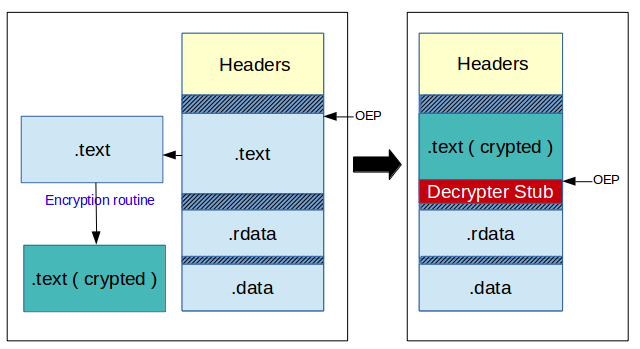
\includegraphics[width=1.1\textwidth]{pictures/packer_general.png} \\\\

Malware writers can decide to use an \textit{off-the-shelf} packer ( commercial or free ) or to implements their own solution with a \textit{custom packer}.

The complexity of \textit{packers} can be very different: from those which write and execute directly the original code, to others that employ multiple unpacking routines and obfuscation techniques such as runtime repacking of previously unpacked code.\\
This process has different consequences both in the AV detection and manual analysis of malicious binary:
\begin{itemize}
\item Usually AV employ different static analysis techniques in order to understand if a file is malicious or not, but packing a binary destroys any possibility to understand what the program will do on the system without executing it, and so void any effort from the point of view of a static analysis.
\item The process of reverse engineering a packed malware can be very time consuming and since lots of malware is pushed every day on the internet there is the necessity of fast analysis and fast updating of AV software.
\end{itemize}
\paragraph{}
These problems inspired different works in building an automatic generic unpacker aimed to extract the original code from the packed one. Some of them are more oriented in detection of malicious packed program helping an AV software on end users PCs, others are instead proposed as tools for speed up the work of professional malware analysts.
\paragraph{}
A comprehensive study and a taxonomy of the levels of complexity of nowadays packers have been presented by Ugarte-Pedrero et al\cite{sokpacker}. 
In order to clarify better what a packer is and how it operates we will discuss in the next capther the main points of the previously mentioned research.

\subsection{Packer taxonomy}
\paragraph{}
As previously explained a packer can implements different obfuscation techniques in order to harden the analysis of a program. In this capther we are going to analyze the proposed taxonomy in order to better understand the goals of our work and its limitation against the current packing methods.

Before starting to present the techniques we need to define some terms that are essential in order to understand how a packer works: 
\begin{itemize}
\item \textit{Layer}: a layer is a set of contiguous memory addresses that are executed after being written.A layer can unpack another unpacking-layer or layer that contains the original program code.
\item \textit{Transition}: a transition is a control transfer from a layer to another layer, it can be a \textit{forward transition} if the execution is going from a previously unpacked layer to a newer layer, or a \textit{backward transition} if the execution is going from a newer layer to an older one. From this definition we can derive the concept of \textit{linear unpacking} in which all the transition are \textit{forward transition}, and {cyclic unpacking} in which there are some \textit{forward transition} and some \textit{backward transition}. 
\item \textit{Tailed/Interleaved}: We say that a packer is tailed if there is soon or later a transition from the unpacking layers to the original program code and then the execution never returns to the unpacking layers, contrary we say that the unpacking is \textit{interleaved} if the execution bounce between the unpacking layers and the original program code. 
\item \textit{Frame}: a frame is a portion of original program code unpacked and executed. If a packer is \textit{mono frame} that means that the unpacking routine will reveal all the original code before jumping and executing it; contrary a \textit{multi frame} packer unpacks only a slice of the original program code, execute it and then unpack another slice of original program code and so on. A \textit{multi frame} behavior can be \textit{incremental} if the slices of original program are revelead in order following the original program execution and never re-encrypted again, contrary a \textit{shifted frames} policy reveal only one slices at times and re-encrypt the slice once executed.
\end{itemize}

As proposed by Ugarte-Pedrero et al\cite{sokpacker} we are going to identify the complexity of a packer by using a scale from 1 to 6.

\subsubsection{Type 1 packer}

The simplest form of packers are \textit{single layer}, they runtime unpack the original binary using a single stub and then jumps to it with a tail jump. 

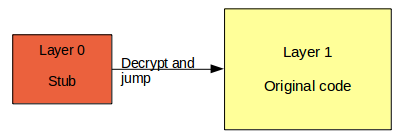
\includegraphics[width=0.7\textwidth]{pictures/packer_type_1.png} 

This scheme is typical of packers like UPX,EXEpacker.

\subsubsection{Type 2 packer}

The packer in this category are defined as \textit{multi-layer} and \textit{linear}. This means that they employ different layers and the transitions between them are always from the older to the newer. Also this kind of packers are defined as \textit{tailed} since the last jump redirect the execution at the original program code.

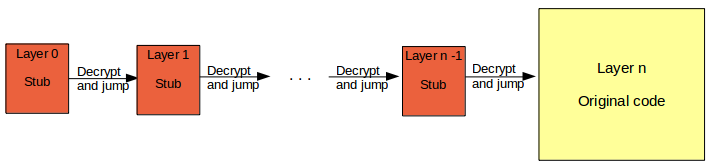
\includegraphics[width=1\textwidth]{pictures/packer_type_2.png}

We can see from the picture that the layer 0 unpack and jumps to the layer1, then the scheme is repeated untill the layer(n-1) that decrypts and finally jumps to the original code. All the layer from 0 to n-1 are part of the packer stub.

\subsubsection{Type 3 packer}

These packers are defined as \textit{multi-layer}, \textit{cyclic} and \textit{tailed}. This means that they employ different layers and the transitions are both \textit{forward transition} and \textit{backward transition}.  

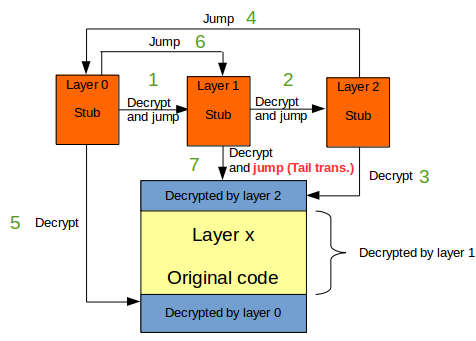
\includegraphics[width=0.9\textwidth]{pictures/packer_type_3.png} 

Following the number reported on the picture let's explain briefly how the process of the packer's stub works in this example of packer type 3, keep in mind that the scheme can change but the properties for this kind of packers remains the one described previously.

\begin{itemize}
\item (1) The first layer decrypt and finally jump to the layer 1.
\item (2) The layer 1 do the same thing, unpacking and jumping to the layer 2.
\item (3) Then the layer 2 decrypt a piece of original program code, and then (4)re-jump with a backward transition to the layer 0.
\item (5) Now the layer 0 decrypt another piece of the original program code and then (6)re-jump to layer 1.
\item (7)Finally layer 1 decrypt the last piece ( Layer X ) of original code and jump to the OEP of the program.
\end{itemize}

A scheme of this type is implemented by PE-Compact, Aspack, FSG, ASprotect,NSPack,WinUpack,UPolyX and Obsidium.

\subsubsection{Type 4 packer}

These packers are \textit{multi-layer}, \textit{cyclic} and \textit{interleaved}. This means that they use different layers with both \textit{forward and backward transitions}, and during the execution of the original program the control is redirected in some way to the packer code.

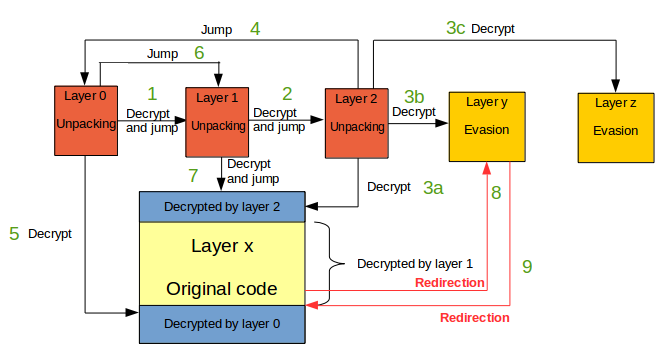
\includegraphics[width=1.07\textwidth]{pictures/packer_type_4.png} 

\begin{itemize}
\item (1) The first layer decrypts and finally jump to the layer 1.
\item (2) The layer 1 do the same thing, unpacking and jumping to the layer 2.
\item (3a) The layer 2 decrypts a piece of original code and (3b+3c)two additional layers that will implement, for example, some evasion techniques like debugger detection. After this (4) it jumps with a backward transition to layer 0.
\item (5) Now layer 0 decrypts another piece of original program and then (6) jumps to layer 1 again.
\item (7) Layer 1 finally decrypts and jump to the original program OEP.
\item (8) During program execution the packer re-gain control executing the evasion routines; this is usually implements by hijacking the API called by original program.
\item (9) After the evasion code has been executed the execution can resume to the original program code or into other location based on the results of the evasion checks implemented.
\end{itemize}

A scheme of this type is implemented by ACProtect.


\subsubsection{Type 5 packer}

Packers of this type are \textit{multi-layer}, \textit{cyclic},\textit{interleaved} and \textit{multi frame} with an \textit{incremental frames} behavior. This means that they use different layers with both \textit{forward and backward transitions}, during the execution of the original program the control is redirected in some way to the packer code and the original program code is revelead slice by slice when need to execute; Like the previous packer's type also here exists a moment in which all the original program code is unpacked in memory, but differently in this case dumping at the OEP doesn't permit to dump all the original program code since it is still encrypted in memory; nonetheless a theoretical dump nearly the end of execution can dump the entire program's code.

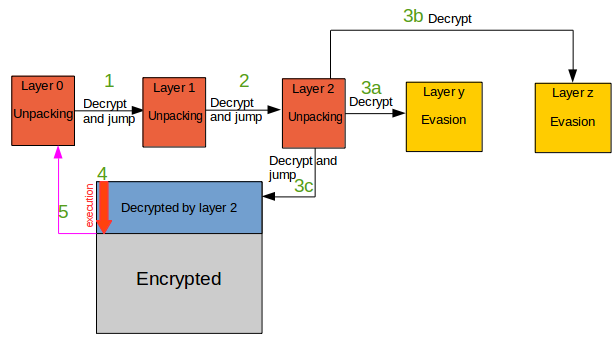
\includegraphics[width=1\textwidth]{pictures/packer_type_5-1.png}

\begin{itemize}
\item (1) The layer 0 unpacks and jumps to layer 1.
\item (2) The layer 1 unpacks and jumps to layer 2.
\item (3a+3b) Layer 2 unpacks two additional layers that will implements some kind of evasion techniques. Finally (3c) it unpacks a slice of original program's code at the OEP and redirect the execution there (4)starting to execute the original program.
\item (5) The execution reach the end of the unpacked original program's code and supposedly an exception will be launched. The packer catches this exception and redirect the execution to layer 0.
\end{itemize}

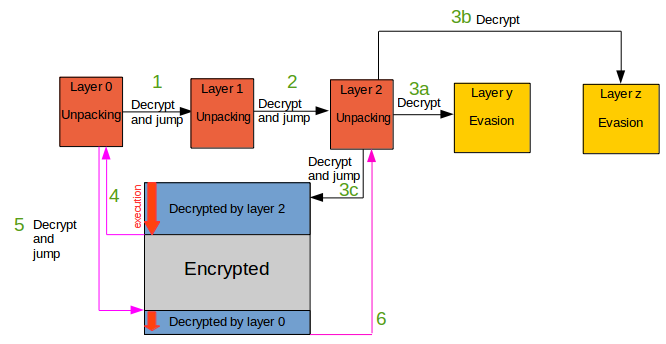
\includegraphics[width=1.1\textwidth]{pictures/packer_type_5-2.png}

\begin{itemize}
\item (5) Layer 0 decrypts on demand a new slice of original program's code and then jumps to it.
\item (6) The same things as before happen when execution reachs again the end of the previously unpacked code, and now the layer 2 take control.
\end{itemize}

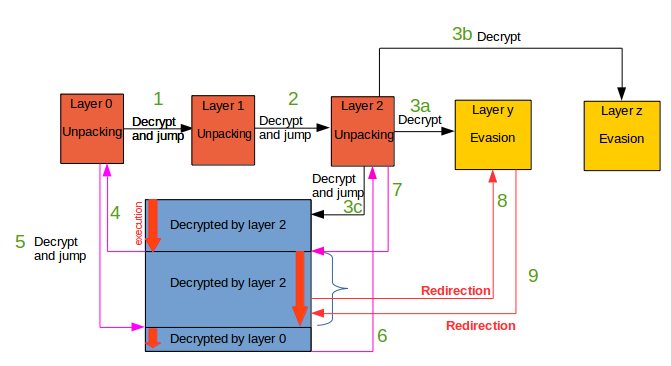
\includegraphics[width=1.1\textwidth]{pictures/packer_type_5-3.png}

\begin{itemize}
\item (7) Layer 2 decrypts the last slice of original program's code and finally jumps to it. As before in (8) there is a redirection to an evasion layer that can decide to (9) resume the execution to the original program's code, or to abort the execution depending on its checks.
\end{itemize}

\subsubsection{Type 6 packer}

Packers of this type are \textit{multi-layer}, \textit{cyclic}, \textit{interleaved} and \textit{multi frame} with a \textit{shifted frames} behavior. This means that they use different layers with both \textit{forward and backward transitions}, during the execution of the original program the control is redirected in some way to the packer code and the original program code is revelead slice by slice and re-encrypted once executed; packers with such complexity never let all the program code to live in memory, so a dump that encompass the entire original program's code doesn't exists.

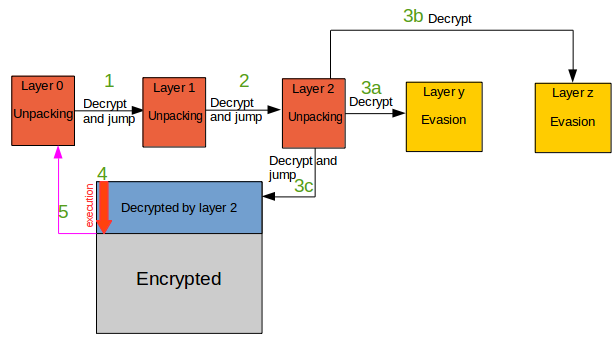
\includegraphics[width=1\textwidth]{pictures/packer_type_5-1.png}

\begin{itemize}
\item (1) The layer 0 unpacks and jumps to layer 1.
\item (2) The layer 1 unpacks and jumps to layer 2.
\item (3a+3b) Layer 2 unpacks two additional layers that will implements some kind of evasion techniques. Finally (3c) it unpacks a slice of original program's code at the OEP and redirect the execution there (4)starting to execute the original program.
\item (5) The execution reach the end of the unpacked original program's code and supposedly an exception will be launched. The packer catches this exception and redirect the execution to layer 0.
\end{itemize}


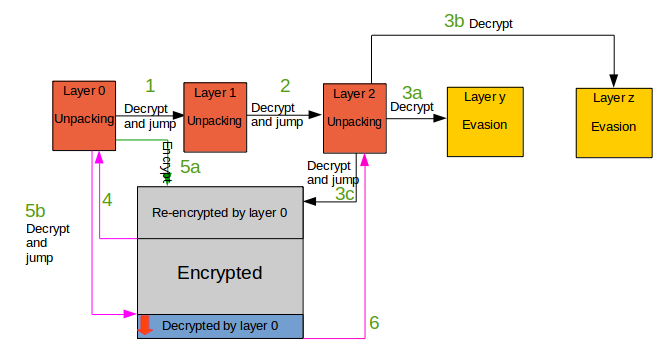
\includegraphics[width=1.05\textwidth]{pictures/packer_type_6-1.png}

\begin{itemize}
\item (5a) Layer 0 re-encrypts the previous slice of original program's code, and (5b) decrypts on demand a new slice of original program's code; finally it jumps to the new unpacked slice.
\item (6) The same things as before happen when execution reachs again the end of the previously unpacked code, and now the layer 2 take control.
\end{itemize}

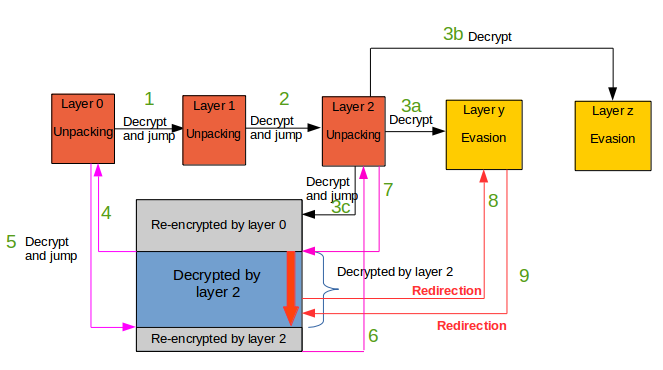
\includegraphics[width=1.05\textwidth]{pictures/packer_type_6-2.png}

\begin{itemize}
\item (7) Layer 2 re-encrypts the previous slice of original program's code and decrypts the last slice, jumping to it at the end. As before in (8) there is a redirection to an evasion layer that can decide to (9) resume the execution to the original program's code, or to abort the execution depending on its checks.
\end{itemize}

A scheme of this type is implemented by Armadillo.

\subsubsection{Packer complexity distribution}

According to Ugarte-Pedrero et al\cite{sokpacker}, the distribution of packer complexity resulted from the analysis of 6088 packed malware binaries is the following:

\begin{table}[H]
\begin{center}
\begin{tabular}{l*{6}{c}r}
Type      & Off-the-shelf & Custom packers \\
\hline
Type 1 &       173 (25.3\%) & 443 (7.3\%) \\
Type 2 &       56 (8.2\%) & 752 (12.4\%) \\
Type 3 &       352 (51.4\%)  & 3993 (65.6\%) \\
Type 4 &       86 (12.6\%) & 843 (13.8\%) \\
Type 5 &       6 (0.9\%)  & 46 (0.8\%) \\
Type 6 &       12 (1.8\%) & 11 (0.2\%) \\
\end{tabular}
\end{center}
\end{table}

Interpreting the data we can derive that:
\begin{itemize}
\item Malware writers seems to predilige using a custom packer rather than rely on an existing one.
\item more than 90\% of the binary packed with both an off-the-shelf/custom packer use a complexity that range from 1 to a maximum of 4. This suggest that a generic unpacker that can handle such complexities can cover a good number of cases. 
\item In both cases of an off-the-shelf/custom packer we can see that the preferred complexity seems to be a Type 3 packer. This could be an indication that a complexity of that level is enough to defeat the nowadays AV solutions.
\item The use of a complexity greater than IV is rarely used.

As presented, the complexity of a packer can escalate really quickly and building a generic unpacker that can cover all these schemes is a big challenge.

\section{State of the art}
\paragraph{}
Lots of different tools using different approaches and techniques have been proposed. 
The approaches for automatic unpacking can be very different:
\begin{itemize}
\item \textit{Static unpacking}: this can sound counterintuitive, but some works proposed to identify unpacking routines inside the binary and reconstruct an ad hoc unpacker for the binary starting from these routines. This approach has got numerous limitation but can lead to interesting result in some case as demonstrated by Coogan et al.\cite{coogan}
\item \textit{Hybrid unpacking}: this mixes some static heuristics with dynamic analysis.
\item \textit{Dynamic unpacking}: these techniques follow the idea to let the unpacker do its work and then try to extract runtime the unpacked code. 
\end{itemize}
\paragraph{}
Depending on the purpose of the tool there are different requirements that a generic unpacker must respect. If the aim is to help the AV on end users' PCs:
\begin{itemize}
\item Safety: try to recognize the malicious behaviour as fast as possible and block the execution. 
\item Performance: it should not slow down too much the execution of AV scans.
\end{itemize}
Note that in these cases, the scope is not to reconstruct a binary from a packed one, but rather to stop malicious behaviours when they manifest. \\
In this area have been done works such as OmniUnpack and JustIn.
\paragraph{}
On the other side if the aim is to help the analysis in a laboratory:
\begin{itemize}
\item Fidelity: the unpacked binary extracted by the tool should be equal to the one that would be unpacked normally. 
\item Generality: the unpacker can not be focused only against one packer but should unpack different of them with one generic algorithm.
\end{itemize}
In this case we do not care so much about safety because usually analysis is performed inside a controlled environment and the analysts want to observe the complete execution of malware. Also the performances are not a critical feature here because we are not constrained by user experience needs.\\
In this category have been developed tools like PolyUnpack, Ether, Eureka, Renovo, Lynx.
These tools merely collect dumps of the binary while unpacking and they don't reconstruct a fully runnable binary given a packed one.


\section{Goals and challenges}
\paragraph{}
Since our work is born as a component of a bigger malware analysis platform (Jackdaw), our tool is oriented to help malware analyst during the reversing process of a packed binary. 
Our approach aims not only to unpack the malware, but also to reconstruct a fully working unpacked binary. To do so, we not only have to identify the original entry point (OEP) and dump the code at that moment, but we have to find the IAT inside the process and reconstruct a correct import directory in the final PE file.\\
The first thing we have to deal with are the unpacking routines of the packers: every time the execution of the malware comes from a previously written memory area, then it could be a sign that the unpacking stage has finished or that a new unpacking layer has started.\\
We have also to deal with techniques of IAT obfuscation: some malwares can do this in order to make difficult to statically analyse them to understand what they are doing.

